        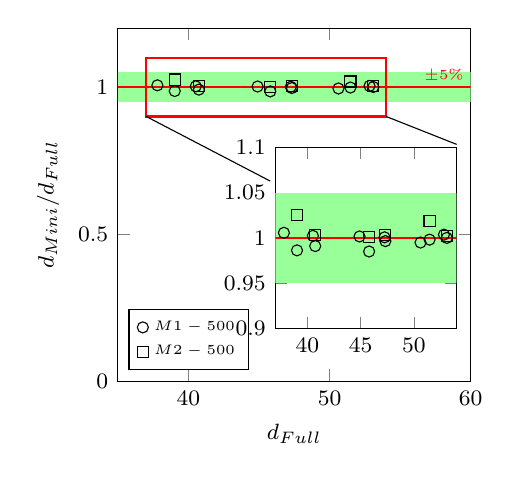
\begin{tikzpicture}[]
        \centering
        \begin{axis}[
            ylabel={$d_{\text{Mini}}/d_{\text{Full}}$},
            xlabel={$d_{\text{Full}}$},
            ymin=0, ymax=1.2,
			xmax=60,
			xmin=35,
			%xtick={-2,-1.5,...,-0.4},
            width=.5\linewidth,
            height=.5\linewidth,
            label style={font=\footnotesize},
            legend style={font=\tiny,anchor=south west},
                        legend pos=south west,
            tick label style={font=\footnotesize}
            ]
			\addplot [
            black,only marks,mark=o,
            ]
            coordinates{
            (40.74,40.38/40.74)
            (39.03,38.50/39.03)
            (40.52,40.62/40.52)
            (37.80,38.02/37.80)
            (47.33,47.17/47.33)
            (45.80,45.12/45.80)
            (47.25,47.29/47.25)
            (44.90,44.90/44.82)
            (53.10,53.11/53.10)
            (51.48,51.39/51.48)
            (52.83,53.03/52.83)
            (50.63,50.38/50.63)
            };
			\addlegendentry{$M1-500$}
			\addplot [
            black,only marks,mark=square,
            ]
            coordinates{
            (40.74, 40.87/40.74)
            (39.03, 40.02/39.03)
            (47.33,47.47/47.33)
            (45.80,45.84/45.80)
            (53.10,53.23/53.10)
            (51.48,52.45/51.48)
            };
			\addlegendentry{$M2-500$}
	
			 \fill[color=green!40,opacity=40] (0,1.05) -- (70,1.05) -- (70,0.95) -- (0,0.95) -- cycle;
			 			%\fill[color=yellow!40,opacity=40] (0,0.18) -- (9,9.18) -- (9,8.82) -- (0,-0.18) -- cycle;
			\addplot [
            red,thick,solid,mark=square,
            ]
            coordinates{
            (30, 1)
            (70, 1)
            };
            \draw[color=red,thick] (37, 0.9) rectangle (54, 1.1);
			\node[red,right] at (axis cs: 56,1.04) {\tiny $\pm5\%$};
  \coordinate (AR1) at (37, 0.9);
        \coordinate (AR2) at (45.8, 0.68);
        \coordinate (AR3) at (54, 0.9);
        \coordinate (AR4) at (59, 0.805);
         \draw[-] (AR1) -- (AR2);
         \draw[-] (AR3) -- (AR4);
        \end{axis}
        
                \begin{axis}[
            %ylabel={$\frac{\Delta U_{Mini}^+}{\Delta U_{Full}^+}$},
            %xlabel={$\Delta U_{Full}^+$},
            ymin=0.9,ymax=1.1,
			xmax=54,
			xmin=37,
			%xtick={-2,-1.5,...,-0.4},
            width=.32\linewidth,
            height=.32\linewidth,
            label style={font=\footnotesize},
            tick label style={font=\footnotesize},
            at={(0.165\linewidth,0.055\linewidth)}
            ]
			\addplot [
            black,only marks,mark=o,
            ]
            coordinates{
            (40.74,40.38/40.74)
            (39.03,38.50/39.03)
            (40.52,40.62/40.52)
            (37.80,38.02/37.80)
            (47.33,47.17/47.33)
            (45.80,45.12/45.80)
            (47.25,47.29/47.25)
            (44.90,44.90/44.82)
            (53.10,53.11/53.10)
            (51.48,51.39/51.48)
            (52.83,53.03/52.83)
            (50.63,50.38/50.63)
            };
			\addplot [
            black,only marks,mark=square,
            ]
            coordinates{
            (40.74, 40.87/40.74)
            (39.03, 40.02/39.03)
            (47.33,47.47/47.33)
            (45.80,45.84/45.80)
            (53.10,53.23/53.10)
            (51.48,52.45/51.48)
            };

			 \fill[color=green!40,opacity=40] (0,1.05) -- (70,1.05) -- (70,0.95) -- (0,0.95) -- cycle;
			 		%	\fill[color=yellow!40,opacity=40] %(20,20.1395/20) -- (60,60.1395/60) -- %(60,59.8605/60) -- (20,19.8605/20) -- cycle;
            \addplot [
            red,thick,solid,mark=square,
            ]
            coordinates{
            (0, 1)
            (90, 1)
            };
			\node[red,right] at (axis cs: 55,1.04) {\tiny $\pm5\%$};
					 			
        \end{axis}
        \end{tikzpicture}